\chapter{Problem analysis \& Objectives}
\section{Analysis}

After confirming that other avenues of control, such as the data port on the back of the device did not provide enough control \footnote{The data port only allows input and output of audio, transfer of station memory when the radio is in a special mode and control of squelch level.}, it became clear that the only way to interface with the radio without opening up the case (and invalidating the warranty) was to utilise the serial line that connects the head and body of the radio.

Previous work on understanding the serial protocol between the body and head of the radio was undertaken by Ben Cooper \cite{ben_report}. \todo{Add Ben Cooper's main source here too}. This work helped me to ascertain the basics of the serial communication. Ben Cooper's project as focused on developing software aimed to run on Arduino microcontrollers. He concludes that the severe complexity of sending, receiving and processing on a single thread was perhaps reason to consider other options.

My aim is to run the project on as many platforms as possible at the lowest cost. For this reason I chose the project to be portable for at least the x86 and ARM architectures. This gives the user as many options as possible, for example low power PC's such as the Raspberry Pi, as well as controlling the radio straight from a laptop that has serial capabilities. This makes development very straightforward with the use of a USB \gls{ttl} dongle. These dongles are cheap and ubiquitous, costing less than \pounds1 each. This could be the only dedicated hardware required for most users.

\subsection{Protocol}
This is primarily a summary of Ben Cooper's work\cite{ben_report} on the transmission protocol as well as some of my own observations. I have been able to confirm these assumptions using a digital oscilloscope. Furthermore I was able to decode both \gls{tx} and \gls{rx} using this method.

The connectors at each end of the serial line are RJ25 ports. These ports have 6 connectors. In the order of left to right from the perspective of looking into the socket, the first 2 lines are for \gls{rx} and \gls{tx} of serial, ground, 9v power, power switch and the last line is for the microphone. 

The radio does not use the common RS232 standard\footnote{RS232 sends binary with -13V to represent a one bit and +13v for a 0 bit, allowing for easy knowledge of when the line is idle at 0V} instead it uses the older \gls{ttl} standard. In this case this means that an idle line is at 5V which represents a 1 bit and 0V representing 0 bit. The beginning of a transmission is marked with a single start bit, followed by 8 bits of data and then a single stop bit. There is no error checking through parity or otherwise. 

So to summarise the communication: 
\begin{itemize}
    \item 0-5V
    \item \gls{ttl} protocol
    \item 8 data bits with 1 stop bit
    \item The most significant bit is transferred first
    \item 19,200 baud rate
    \todo{include packet timings}
\end{itemize}

\gls{tx} from the head to the body of the radio does two things. For analog buttons it transmits the current state of those buttons and for digital encoders, such as the dials, it transmits the number of rotations since the last \gls{tx}. The packet of data that is sent consists of 13 bytes (mapped previously\cite{ben_report}). This could be utilised as a method to provide emulated input to the radio. Actions could be undertaken by the program to replicate any input that a human was capable of.

\begin{figure}
    \centering
    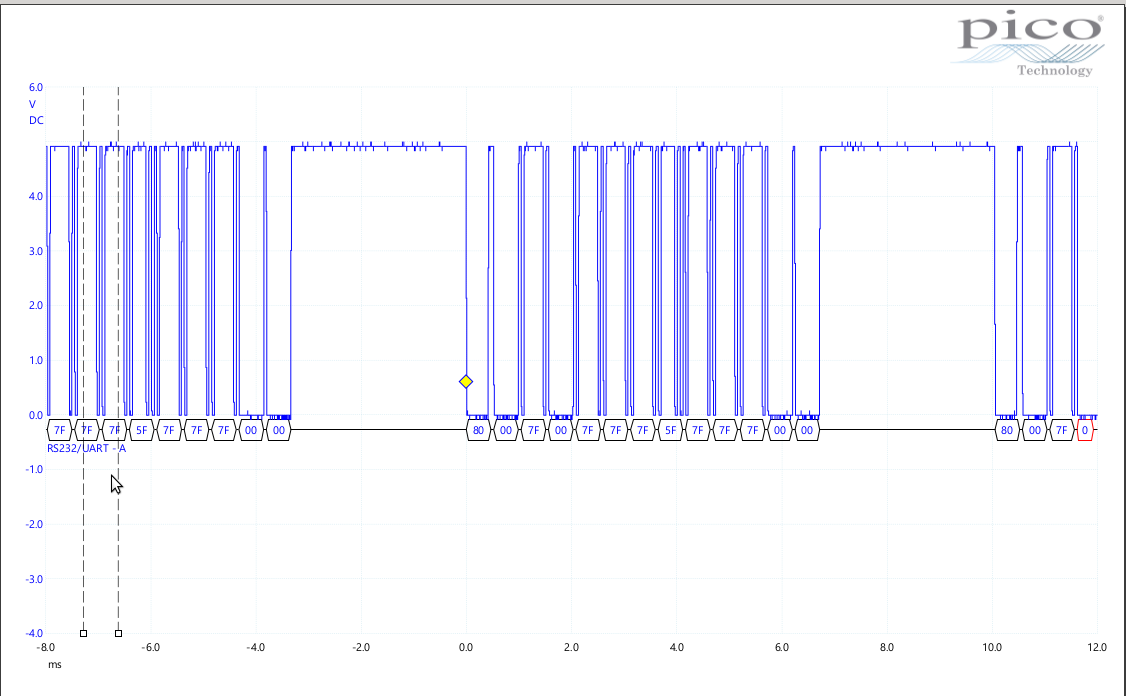
\includegraphics[width=1\textwidth]{img/controll_packet.png}
    \caption[Control packet]{A capture of control packets. The 2 long peeks are the begging and end of the middle packet}
    \label{fig:control_packet}
\end{figure}

\gls{rx} (from the body to the head) is a packet of 42 bytes. Each bit in the packet represents whether a segment of the screen should be illuminated or not, for example what frequency should be shown. The program can listen to this to learn the internal state of the radio. State that is not shown regularly would have to be discovered by navigating the menus and then reading the screen.

I was also able to measure the timings of the packets. \todo{add packet times here}

\section{Aim \& Deliverables}
The scope of my development efforts will be to create a way to control the body of the radio, with the aim to achieve as much functionality as possible (controllable by a computer). Communication to the head, for the purposes of using the head as a generic control surface will remain out of scope. This non-critical feature would be at a high cost in time spent, when instead more important control features could be implemented. However the work done will be foundational to this feature if desired later. Dealing with the audio from the radio was deemed out of scope as the data-port of the back of the radio can already achieve this. With the use of a cable speaker line out and microphone line out is given.

Below is a list of deliverables. Necessary functions were derived by asking a number of ``Customers'' what they would consider their minimum set of features (aka the planning game) and there expected difficulty. They are also in order of priority. Therefore this became was my priority backlog.

\begin{itemize}
    \item Final report
    \item Software functions that have been deemed necessary for radio control:
        \subitem Frequency
        \subitem Push to talk
        \subitem Volume
        \subitem \gls{squelch}
        \subitem Power
        \subitem Powering on the radio
    \item Documentation
        \subitem Code documentation (\gls{doxygen})
        \subitem Schematic of prototype serial controller
\end{itemize}

Futures as a more permanent printed circuit board and control of all functions of the radio were deemed not possible in the allotted semester of work\footnote{From \formatdate{30}{01}{2017} to \formatdate{08}{04}{2017}.}. Originally I expressed my intent on providing a patch to the open source Ham Radio Control Libraries, Hamlib\cite{hamlib}. The Initial report outline submitted reflected this. However after discussion of my intent on the developer mailing list it became clear that a multi-threaded application was unacceptable within the Hamlib codebase, due to concerns with portability and stability. Instead future work will likely include some sort of inter process communication through a socket.

\section{Security}
The envisioned scope of the project means that the software will not be networked in the modern sense of using IP communication. Operating systems manage access to serial communications often by requiring special privileges or groups. Therefore in this case, loss of access control can be prevented using just the default system configuration of most operating systems. The application will endeavour to not manipulate the system as much as is possible so as to minimise the attack surface given. Attention will be given to proper copying in memory and validation of incoming received serial communications to mitigate fuzzing based attacks.

Considerations will have to be made on who has physical access to the computer connected to the radio. As another user could plug the serial connection into their computer in order to interface with it, thereby forgoing the access control in place on the system. Users will also have to consult their local laws on whether it is legal for them to operate their radio remotely in their respective countries. 

\section{Process}
My intent was to use the most appropriate agile software development methodology for the project. I considered Scrum, \gls{xp} and \gls{fdd}. I quickly ruled out \gls{fdd} as it often works best with larger teams that need to be able to produce lots of status reports. For my project I feared that this would slow down the rate of my development of features. I saw scrum as less useful for me than \gls{xp} as it does not talk about the actual engineering steps to take in programming unlike \gls{xp} does. Instead it focuses more as general a way to manage a team. 

\gls{xp} guidelines for design can be summarised to the following\cite{xp}:
\begin{itemize}
    \item The Planning Game 	
    \item Small Releases (Iterations)
    \item System Metaphors
    \item Simple Design 	
\end{itemize}
These points make sense for the lone developer project. The customer can be any potential user of the radio. When possible I used the planning game with potential ``customers'' i.e with my supervisor, by asking him to prioritise the feature list of the radio. I did this using \gls{crc} cards, with the acceptance tests on the back of the cards. 

\todo[inline]{make some scans of \gls{crc} cards to place here}

Evidence of my use of system metaphors can been seen in this report with the ``head'' and ``body'' metaphors or standardisation of point of reference to serial communication with the \gls{rx} and \gls{tx}  terms. Small releases make sense so that they can be tested with the real hardware as much as possible\footnote{Working next to the radio was not always possible as the radio was stored in a university lab that was shut on the evening, Fridays and weekends.}. My initial design of the application will be just large enough to start development without the need for heavy refactoring later. 

The actual development methods used in \gls{xp} will need to be modified in order to accommodate one developer. Thankfully adaption to a single developer as been discussed openly, including from the creator of \gls{xp}, Kent Beck in a number of mailing list discussions\cite{xpforone}\cite{lone_developer}.

The following sections will address my adaptations:
\subsection*{Unit Tests}
The described use of unit tests do not need to be changed for the project. The test suite that I have chosen is ``Google Tests''\cite{google_tests}. Despite the fact that this is implemented in C++ it is often used to test C code as it has better community support than native suites. Its test macros are familiar to programmers that have used suites such as JUnit etc.  

\subsection*{Acceptance Tests}
Acceptance Tests are created on the back of \gls{crc} cards. A successful test is likely to be the ability for the user to preform said action on the real radio without any input from the developer.

\subsection*{Refactoring}
Refactoring will occur naturally throughout development and in the refactoring stage of creating a function with the \gls{rgf} method. Good use of unit tests will make refactoring easier as developers can make changes with confidence of not braking the system.

\todo[inline]{add references to actual XP methodology}

\subsection*{Pair Programming}
\gls{xp} has a heavy focus on pair programming. For this project I am not permitted to work this way in order for a full assessment to take place of my work done. Instead I will try other methods that give some of the benefits of group collaboration such as``rubber ducking''. This is the process of talking out or explaining code in order to check that there are not better ways to do something. Throughout the project I also conversed with other students about what I was working on, for example when walking up to campus. This was beneficial as questions from others asking why I did something in a particular way can promote further analysis and better ideas.

\subsection*{Continuous Integration}
I will be using Git as a VCS for the project, \todo[]{add reasoning}. I will work using the centralised repository workflow and use branches for new features before merging them. To host the central repository I will use Github, due to its good user interface as well as its large popularity (meaning new user discovery is possible). From there I will run my own Jenkins \todo[]{refrence this (https://jenkins.io/)} instance. I chose the open source Jenkins CI due to my previous positive experiences with it including its large plugin library making it very customisable. 

\subsection*{Coding Standards}	
I chose the ``Linux kernel coding style''\cite{linux_coding_style} as it is a widely used standard that has a good rationale and format. To enforce constant code I have added style checking to my editor, as well as a step in my continuous integration checks to look for style violations.

\subsection*{Iterations}
For my project I have chosen a two week release cycle. I hope this will give enough time to plan, develop, and physically test the radio functions. In this time I will work on the current most needed feature from the priority backlog. To do this I will make a number of engineering tasks. I placed these tasks as ``TODO'' items in my source code. I believe this is the most appropriate place as tasks remain very visible until removed, unlike if when tasks are recorded on a webpage elsewhere.  At the end of an iteration I will tag a release in git using the a version number that conforms to the semantic versioning convention\cite{sem_ver}. Additionally I will make a changelog on my developer blog. This means there are regular versions of the software that can be tested.
